\section{Introduction}

	\subsection{Goal}
		The goal of this experiment is to observe the particle properties of light and to analyze the experimental observations to validate the wave-particle duality, bridging the gap between classical and quantum physics. 
	
	\subsection{Theory}
		
		\paragraph{Thomson Scattering - Classical Electromagnetic Theory}
			Thomson scattering is an example of elastic scattering of electromagnetic radiation. The electric and magnetic fields components of an electromagnetic field exerts a Lorentz force on a particle, which sets it into motion that is periodic in time. Since the particle is now accelerated, it emits radiation.
			\\
			\\
			The electric field component of a linearly polarized, monochromatic, plane wave incident on a particle of charge \textbf{q} can be written as 
			\begin{equation}	E = e E_0 exp(i (k.r - wt))
			\end{equation}
			The particle undergoes oscillations with small amplitude, therefore its velocity is assumed to be non-relativistic, enabling us to neglect the magnetic component of the Lorentz force. Then the EOM of the charged particle can be written as  
			\begin{equation}
				F = q E = m \ddot{s}
			\end{equation}
			where \textbf{s} is the displacement from the origin. 
			\\
			\\
			Then the time averaged power radiated per unit solid angle becomes
			\begin{equation}
				\frac{d P}{d \Omega} = \frac{q^2 <\ddot{s}^2>}{16 \pi^2 \epsilon_0 c^3} sin^2 \theta
			\end{equation}
			and
			\begin{equation}
				<\ddot{s}^2> = \frac{q^2}{m^2} <E^2> = \frac{q^2 E_0^2}{2 m^2}
			\end{equation}
			Which essentially means that the oscillating particle acts as a short antenna.
			\\
			\\
			The resulting radiation will be perpendicular to the acceleration of the particle and be polarized along its direction of motion. 
			\\
			\begin{figure}[h]
				\caption{Thomson Scattering Diagram}
				\centering
				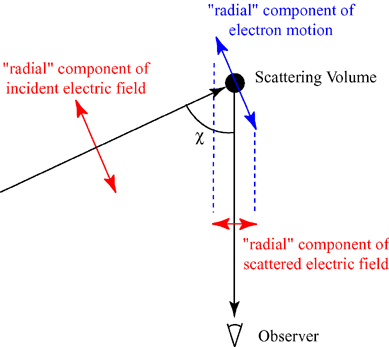
\includegraphics[width=\textwidth / 2]{images/thomson_scattering.png}
			\end{figure}
			
			
		\paragraph{Compton Scattering - Particle Properties Of Light}
		Compton scattering is an example of inelastic scattering of electromagnetic radiation. Collision between a photon $\gamma$ with wavelength $\lambda$ and an electron $e$ that is at rest causes the electron to recoil, which in turn results in a new photon $\gamma'$ with wavelength $\lambda'$ at angle $\theta$ from the incident photon's path. 
		\begin{figure}[h]
			\caption{Compton Scattering Diagram}
			\centering
			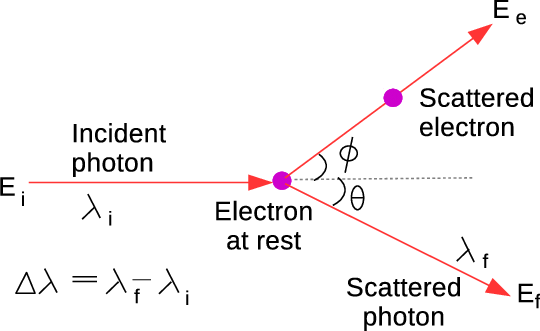
\includegraphics[width=\textwidth ]{images/compton_scattering.png}
		\end{figure}
		Using the conservation of energy, we have
		\begin{equation}
			E_\gamma + E_e = E_{\gamma'} + E_{e'}.
		\end{equation}
		Compton postulated that photons carry momentum and used the conservation of momentum as well
		\begin{equation}
			p_\gamma + p_e = p_{\gamma'} + p_{e'}
		\end{equation}
		Knowing that,
		\begin{equation}
			E_\gamma = h f \text{, } E_{\gamma'} = h f'
		\end{equation}
		and that,
		\begin{equation}
			E_e = m_e c^2 \text{, } E_{e'} = \sqrt{(p_{e'} c)^2 + (m_e c^2)^2}
		\end{equation}
		We expect the electron to be accelerated to a relativistic speed after the collision, thus we used the relativistic energy and momentum relation.
		\\
		Substituting these variables in the conservation relations, we get
		\begin{equation}
			h f + m_e c^2 = h f' + \sqrt{(p_{e'} c)^2 + (m_e c^2)^2} \text{ and }
			p_{e'}^2 c^2 = (h f - h f' + m_e c^2)^2 - m_e^2 c^4.
		\end{equation}
		Solving the equation for the conservation of momentum,
		\begin{align*}
			p_{e'}^2 c^2 = p_\gamma^2 c^2 + p_{\gamma'} c^2 - 2 c^2 p_\gamma p_{\gamma'} cos\theta, \\
			p_{e'}^2 c^2 = (h f)^2 + (h f')^2 - 2 (h f) (h f') cos\theta, \\
			2 h f m_e c^2 - 2 h f' m_e c^2 = 2 h^2 f f' (1 - cos\theta), \\
			\frac{c}{f'} - \frac{c}{f} = \frac{h}{m c} (1 - cos\theta).
		\end{align*}
		And finally, after rigorous derivation, we arrive at the famous Compton Shift expression
		\begin{equation}
			\Delta \lambda = \lambda' - \lambda = \frac{h}{m_e c} (1 - cos\theta).
		\end{equation}
		Where $\lambda$ is the wavelength of the incident photon, $\lambda'$ is the wavelength of the scattered photon, $m_e$ is the rest mass of the electron, $\theta$ is the scattering angle and the expression $\frac{h}{m_e c}$ is the Compton wavelength. 
		
		\paragraph{Bridging The Gap}
			As it is clear from the derivations, Thomson scattering is the low-energy limit of Compton scattering, where the photon energy is much smaller than the resting energy of the electron $\mu << m c^2 / h$. Since classical electrodynamics fails to explain the wavelength shift between the incident and scattered photons, realization of this phenomena had important implications on physicists' understanding of light since light clearly behaves as if it consists of particles in this experiment. 